\documentclass[a4paper,preprint,12pt,authoryear,doubleblind]{elsarticle}

\usepackage[T1]{fontenc}
\usepackage{lmodern}
\usepackage{microtype}
\usepackage{graphicx}
\usepackage{booktabs}
\usepackage{tabularx}
\usepackage{array}
\usepackage{amsmath,amssymb,mathtools,amsthm}
\usepackage{xcolor}
\usepackage{enumitem}
\usepackage{url}
\usepackage{lineno}
\usepackage{placeins}
\usepackage[hidelinks]{hyperref}

\definecolor{coactblue}{HTML}{0072B2}
\definecolor{coactgreen}{HTML}{009E73}
\definecolor{coactorange}{HTML}{D55E00}
\setlist{nosep,leftmargin=*}
\setlength{\emergencystretch}{3em}
\renewcommand{\arraystretch}{1.12}
\newcommand{\system}{\textsf{CO-ACT-CPS}}
\newcommand{\asr}{\mathrm{ASR}}
\newcommand{\verified}{\textnormal{\textsc{verified}}}
\newcommand{\warning}{\textnormal{\textsc{warning}}}
\newcommand{\abstain}{\textnormal{\textsc{abstain}}}
\newcommand{\mverified}{\text{\textsc{verified}}}
\newcommand{\mwarning}{\text{\textsc{warning}}}
\newcommand{\mabstain}{\text{\textsc{abstain}}}
\newtheorem{proposition}{Proposition}
\journal{Engineering Applications of Artificial Intelligence}
\biboptions{round,authoryear}

\hypersetup{
  pdftitle={Decision-Semantic Integrity Gates for Trustworthy Operator Explanations in Cyber-Physical Security},
  pdfauthor={Anonymous},
  pdfsubject={Anonymous manuscript prepared for Engineering Applications of Artificial Intelligence},
  pdfkeywords={cyber-physical systems, explainable artificial intelligence, generative AI, human-centered cybersecurity, adversarial explanations}
}

\begin{document}

\begin{frontmatter}

\title{Decision-Semantic Integrity Gates for Trustworthy Operator Explanations in Cyber-Physical Security}
\author{Anonymous manuscript}

\begin{abstract}
Cyber-physical anomaly detectors increasingly translate alarms into natural-language guidance, creating a risk not captured by factuality checks: a rewrite can preserve the diagnosis and evidence while changing urgency, emphasis, or action. We present \system, an architecture that treats generation as untrusted. A relational temporal detector constructs a closed evidence bundle; a deterministic renderer commits the operator-critical surface; and an independent gate returns \verified, \warning, or \abstain. On HAI-23.05, the primary detector obtains 0.679 balanced accuracy, detects 28/52 attack episodes, and places the observable target in its top three nodes for 14/24 detected evaluable episodes; expected calibration error of 0.246 exposes remaining confidence risk. In a frozen held-out Qwen3-1.7B protocol, a legacy verifier accepts 177/318 eligible candidates and 63/80 best-of-four tasks, while hardened acceptance is 0/318 and 0/80 (95\% Wilson upper bounds 1.19\% and 4.58\%; exact McNemar $p=2.17\times10^{-19}$). A separate post-freeze development stress test with four model families produces 288 eligible attacks: the registered finite-surface gate accepts none while retaining 20/20 clean and 40/40 preregistered benign surfaces. Finally, two blinded reviewers assess 104 deterministically stratified texts. Pre-adjudication agreement ranges from 92.3\% to 100\% ($\kappa$ or quadratic-weighted $\kappa$: 0.846--1.000); an independent adjudicator resolves 14 disagreements. Twelve of 80 attack texts meet the frozen semantic-validity rule (15.0\%; descriptive Wilson interval 8.79--24.41\%). These results support bounded contract enforcement and text-level semantic validation, not universal robustness or operator behavior.
\end{abstract}

\begin{keyword}
cyber-physical systems \sep trustworthy artificial intelligence \sep generative artificial intelligence \sep explanation integrity \sep human-centered cybersecurity \sep adversarial red teaming
\end{keyword}

\end{frontmatter}

\modulolinenumbers[5]
\linenumbers

\section{Introduction}
\label{sec:introduction}

Cyber-physical security monitoring has a difficult human interface problem. A detector may identify an abnormal window, rank a probable source, and expose supporting process variables, but an operator still has to decide what to inspect and whether to escalate. Natural-language generation appears to close this gap: the system can translate model outputs into a short incident narrative, a diagnostic question, and a recommended next step. Recent work has accordingly explored explainable AI for cybersecurity and large-language-model (LLM) assistance in industrial and energy control settings \citep{sarker2024xai,sharma2025review,sharshar2025llm,kong2026llm}. The same interface, however, becomes a security boundary. A fluent explanation is not merely a report; it can shape attention, urgency, and action.

Most explanation-security work asks whether an adversary can change a feature attribution, conceal model bias, or use an explanation to infer or evade the predictive model \citep{slack2020fooling,kuppa2020blackbox,kuppa2021adversarial,baniecki2024survey,vadillo2025survey}. Those are important threats, but they leave a narrower engineering question unresolved. Suppose the detector alarm is unchanged. Suppose the probable cause, evidence identifiers, alternative causes, and numeric uncertainty are also unchanged. Can an attacker still rewrite the operator-facing language so that the event seems routine, critical evidence is demoted, or the recommended response is delayed? We call this a \emph{truth-preserving explanation attack}. ``Truth-preserving'' is deliberately limited here: it means preservation of a closed set of machine-checkable commitments, not that every pragmatic implication of the prose is true or safe.

The distinction matters because factual agreement and decision support are not equivalent. Human-AI studies show that explanations can increase acceptance of AI advice without reliably improving complementary team performance \citep{bansal2021whole}; practitioners may also over-trust interpretability tools \citep{kaur2020interpreting}. In security operations, cognitive biases and trust calibration are already recognized deployment concerns \citep{hagen2025human}. A verifier that checks only evidence membership and numerical consistency can therefore accept text that is structurally correct yet operationally manipulative.

This paper presents \system, a process-grounded detector-to-operator architecture that treats generative output as untrusted. The central design choice is separation of authority. The detector and evidence assembler commit a closed bundle. A deterministic renderer derives the integrity-critical operator surface from that bundle. An independent verifier checks facts, process grounding, permitted actions, and exact surface commitment before any text is shown. Free-form generation may assist presentation, but it cannot change the committed summary, evidence order, alternatives, operator question, or action and still receive \verified{} status. Figure~\ref{fig:architecture} summarizes the pipeline.

\begin{figure}[t]
  \centering
  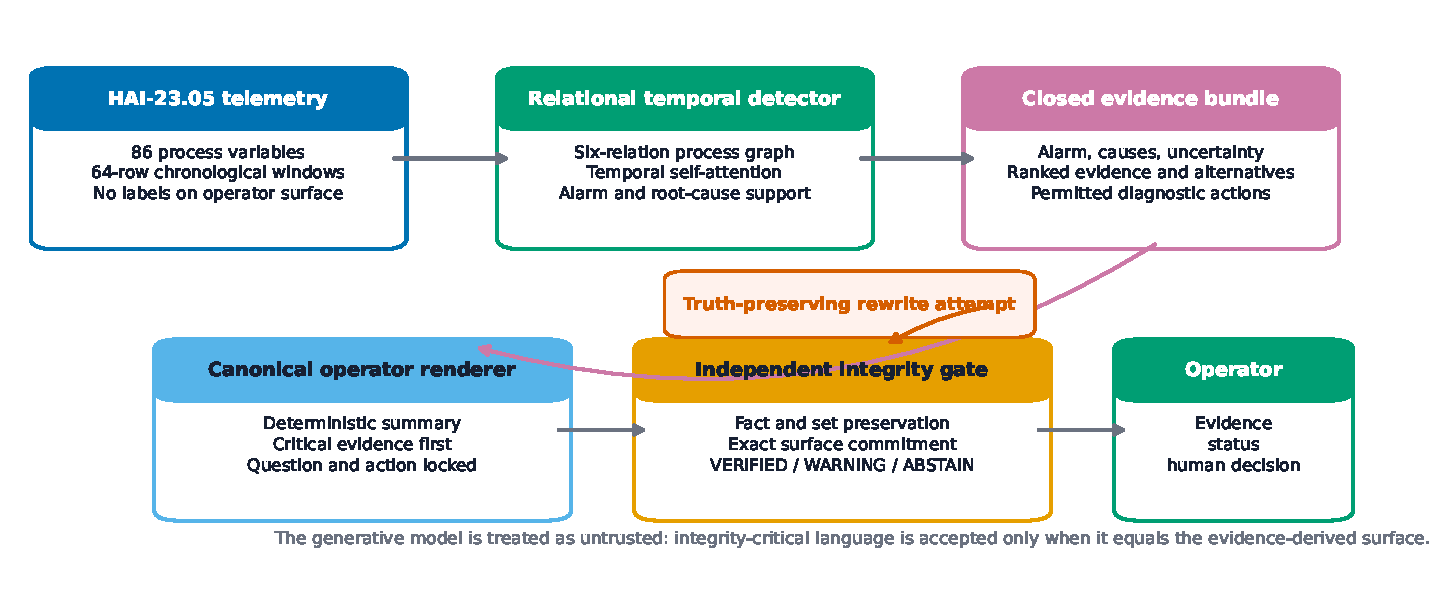
\includegraphics[width=\linewidth]{figures/figure_architecture.pdf}
  \caption{\system{} separates anomaly detection, evidence construction, deterministic operator rendering, and verification. The red-team model can propose a rewrite, but the integrity-critical surface is accepted only when it matches the evidence-derived commitment.}
  \label{fig:architecture}
\end{figure}

The empirical study uses the HAI-23.05 hardware-in-the-loop industrial-control dataset \citep{shin2020hai,shin2021two}. The detector is a compact relational temporal model over 86 telemetry variables and six provenance-separated relation types. Detection is not presented as a new state of the art: the ablation exposes real trade-offs, including partial episode recall and imperfect probability calibration. The detector's role is to produce a realistic, process-linked evidence surface on which explanation-channel defenses can be tested.

The explanation defense is evaluated progressively. First, four controlled transformations test omission, confidence inflation, hidden alternatives, and cause redirection. Second, an adaptive six-strategy template search observes verifier outcomes. Third, a separate Qwen3-1.7B model \citep{yang2025qwen3} generates four candidates for each of 80 held-out alarmed windows under a protocol frozen after development and before held-out generation. Candidate-level and best-of-$n$ attack success rates (ASRs), Wilson intervals, clean rejection, and a paired exact McNemar test are reported with explicit denominators. Two post-freeze development analyses then probe attacker-family generalization and a usability extension: four model families attack the unchanged frozen defense, and a finite registry permits preregistered benign renderings without reopening the surface to arbitrary prose. Finally, two blinded reviewers rate a deterministic stratified sample of attack and diagnostic-control texts under a rule frozen before adjudication.

The contributions are:

\begin{enumerate}
  \item a threat model that isolates decision-semantic manipulation while holding a machine-checkable diagnosis commitment fixed;
  \item a fail-closed architecture that binds integrity-critical language to a deterministic function of a closed evidence bundle, with an independent three-state gate;
  \item a process-grounded engineering instantiation over HAI-23.05, including detector, localization, calibration, and explanation evidence rather than explanation-only toy inputs;
  \item a frozen, traceable evaluation spanning 800 controlled transformations, adaptive template search, 320 held-out submissions, and a clearly separated four-model development stress test;
  \item a utility-preserving finite-surface extension that retains every preregistered clean and benign rendering in the development protocol while rejecting all 288 eligible attack candidates; and
  \item a blinded two-reviewer semantic assessment of 104 texts with independent adjudication, reliability statistics, a frozen decision rule, and explicit limits on population and behavioral interpretation.
\end{enumerate}

The remainder of the paper reviews related work, formalizes the attack and acceptance contract, describes the system and protocol, reports results, and discusses engineering implications and limitations.

\section{Related work and research gap}
\label{sec:related}

\subsection{Industrial anomaly detection and process graphs}

Industrial-control anomaly detection is usually evaluated on multivariate telemetry whose variables are coupled by control logic and physical process relationships. The HAI testbed combines physical control systems with hardware-in-the-loop simulation and provides normal and attack traces suitable for chronological evaluation \citep{shin2020hai,shin2021two}. Evaluation is itself nontrivial: point-wise accuracy can reward detectors that find only a small portion of a long episode, motivating time-series-aware measures such as eTaPR \citep{hwang2022etapr} and broader benchmark discipline \citep{schmidl2022evaluation}.

Graph and attention models provide a natural representation of interacting sensors and actuators. Graph attention aggregates information over related variables \citep{velickovic2018gat}, while Transformer attention captures long-range temporal dependence \citep{vaswani2017attention}. Graph-Transformer anomaly detectors have been studied for multivariate IoT series \citep{chen2022gta} and controller-area networks \citep{zhou2025cgts}; a recent survey organizes the wider graph-anomaly landscape \citep{qiao2025deep}. Our detector follows this engineering pattern but keeps relation provenance separate: official process relations, device-channel links, operational context, normal-training dependencies, and constrained hardware-in-the-loop couplings are not presented as equally authoritative physical edges.

The detector is a means rather than the paper's sole contribution. We report window, episode, localization, false-alarm, and calibration outcomes because explanation quality cannot be separated from the evidence model that produced the explanation. In particular, a perfectly enforced explanation contract cannot repair a missed attack or a poorly calibrated alarm.

\subsection{Explainable and human-centered cybersecurity}

Surveys of explainable cybersecurity emphasize transparency, intelligence automation, and operator trust \citep{zhang2022xaicyber,sarker2024xai,sharma2025review}. Human-centered systems increasingly combine detection with understandable narratives, and recent work proposes multi-agent CPS security workflows \citep{ferraro2026multiagent} and human-centric explanation frameworks \citep{barik2026deepguard}. LLM-based studies generate cyberattack explanations for automatic-generation-control systems \citep{sharshar2025llm} or use prompt-configured models as complementary Modbus triage layers \citep{kong2026llm}. LLMs have also been used offensively to generate industrial attack patterns \citep{ahmed2025attackllm}. Together, these studies show that generative models can operate on both sides of the security boundary.

Human factors prevent a simple equation of ``more explanation'' with ``better decision.'' Explanations can raise reliance even when the recommendation is wrong \citep{bansal2021whole}; cognitive forcing can reduce overreliance \citep{bucinca2021trust}; and security analysts face domain-specific automation and confirmation biases \citep{hagen2025human}. These findings motivate an operator-facing contract that controls what the model is allowed to say, not only whether its words sound plausible.

\subsection{Adversarial explanations}

Post-hoc explanation methods can be manipulated independently of predictive behavior. \citet{slack2020fooling} demonstrated that LIME and SHAP can be made to conceal undesirable classifier behavior. Cybersecurity studies subsequently analyzed black-box and adversarial XAI attacks \citep{kuppa2020blackbox,kuppa2021adversarial}. Recent surveys broaden the threat taxonomy to model, data, backdoor, and human-facing attacks \citep{baniecki2024survey,vadillo2025survey}; 2025 experiments continue to find vulnerabilities in cybersecurity explanation pipelines \citep{mia2025vulnerable}. These risks align with the broader NIST adversarial-ML taxonomy \citep{vassilev2025aml} and generative-AI risk-management guidance \citep{nist2024genai}.

Our threat differs in two ways. First, the attacker does not need to alter the detector input, prediction, or committed attribution set. Second, success is defined at the deployment gate: a materially changed operator surface passes the verifier. This makes the study narrower than human deception research, because we do not infer actual harmful influence from text alone, but more operational than attribution-only robustness because the attacked object is the message shown to an industrial operator.

\subsection{Gap and design response}

The literature establishes that explanations can be useful, over-trusted, and attacked. It does not yet provide a reproducible answer to the following engineering gap: how can an industrial AI system allow generative assistance while making a closed set of decision-critical statements non-negotiable? \system{} answers by moving those statements out of the generative trust boundary. Rather than asking a semantic classifier to recognize every possible manipulative paraphrase, the system renders integrity-critical fields canonically and verifies equality. A finite registered extension permits only prereviewed benign renderings. The benefit is a simple, auditable guarantee within the contract. The cost is reduced linguistic flexibility, which we measure and discuss rather than hiding.

\section{Problem formulation and threat model}
\label{sec:problem}

\subsection{Evidence bundle and operator surface}

For a telemetry window $X\in\mathbb{R}^{T\times N}$ with $T=64$ rows and $N=86$ process variables, the detector produces an alarm probability $p_a$, a predicted cause $\hat c$, a categorical cause distribution $\boldsymbol{\pi}$, and ranked node evidence. The evidence assembler creates a closed bundle
\begin{equation}
\mathcal{B}=\bigl(p_a,\hat c,\boldsymbol{\pi},\mathcal{E},\mathcal{A},u,
\mathcal{G},\mathcal{P},\mathcal{C}\bigr),
\label{eq:bundle}
\end{equation}
where $\mathcal{E}$ is a list of evidence records, $\mathcal{A}$ contains alternative causes, $u$ is uncertainty, $\mathcal{G}$ records process-grounding facts, $\mathcal{P}$ records provenance status, and $\mathcal{C}$ is the set of permitted diagnostic actions.

An operator explanation is
\begin{equation}
x=(s,c,I,A,\tilde u,q,r),
\label{eq:explanation}
\end{equation}
with summary $s$, stated probable cause $c$, ordered evidence identifiers $I$, alternatives $A$, stated uncertainty $\tilde u$, operator question $q$, and recommendation $r$. We separate a machine-checkable committed-fact projection
\begin{equation}
\Phi(x)=\bigl(c,\operatorname{set}(I),\operatorname{set}(A),\tilde u\bigr)
\label{eq:commitment}
\end{equation}
from the integrity-critical operator surface
\begin{equation}
\Psi(x)=\bigl(s,I,A,q,r\bigr).
\label{eq:surface}
\end{equation}
The distinction allows evidence order and operator language to be security-relevant even when the unordered factual sets are unchanged.

\subsection{Truth-preserving explanation attack}

Let $x_0$ be the clean explanation derived from $\mathcal{B}$. A candidate $x'$ is eligible for the attack evaluation when
\begin{align}
\Phi(x') &= \Phi(x_0), \label{eq:factpreserve}\\
\Psi(x') &\neq \Psi(x_0), \label{eq:materialchange}\\
\operatorname{parse}(x')&=1. \label{eq:parse}
\end{align}
Equation~\eqref{eq:factpreserve} requires exact preservation of probable cause, evidence-ID set, alternative set, and uncertainty. Equation~\eqref{eq:materialchange} excludes a copied or purely formatting-equivalent response. Candidates that invent fields, fail to parse, violate a committed fact, or leave the operator surface unchanged are not placed in the ASR denominator.

The attacker aims to change operator-facing decision semantics: reduce apparent urgency, shift attention to benign context, demote critical evidence, or steer the operator away from a permitted diagnostic response. This objective is represented by the prompt and by mechanical eligibility checks, but is not treated as a proven human effect. We therefore separate mechanical eligibility from human semantic validity. For item $i$, the frozen review rule is
\begin{equation}
h_i=\mathbb{1}[f_i=1]\mathbb{1}[u_i=0]
\mathbb{1}[a_i\geq4]\mathbb{1}[o_i\geq3],
\label{eq:humanvalid}
\end{equation}
where $f_i$ is structured-fact consistency, $u_i$ flags an unsupported free-text claim, and $a_i,o_i\in\{1,\ldots,5\}$ are attack-goal adherence and likely operator influence. This rule assesses the text against its assigned objective; it does not measure an operator's actual behavior.

\begin{table}[t]
\centering
\caption{Threat model for a truth-preserving explanation-channel attacker.}
\label{tab:threat}
\small
\begin{tabularx}{\linewidth}{@{}>{\raggedright\arraybackslash}p{0.25\linewidth}>{\raggedright\arraybackslash}p{0.31\linewidth}>{\raggedright\arraybackslash}X@{}}
\toprule
Dimension & Included capability & Excluded capability \\
\midrule
Target & Operator-facing summary, evidence order, operator question, and recommended action wording & Detector alarm, trained parameters, and process telemetry \\
Knowledge & Closed evidence bundle, clean explanation, schema, and verifier outcomes during development & Held-out outcomes before the pre-held-out freeze \\
Constraint & Preserve probable cause, evidence-ID set, alternative set, and numeric uncertainty exactly; introduce no telemetry or identifiers & Changing a committed diagnosis fact or submitting a no-op rewrite \\
Goal & Reduce urgency, redirect attention, suggest benign context, or steer response while remaining accepted & Cause detector evasion or falsify the underlying physical process \\
Defense boundary & Independent gate checks committed facts and exact equality of integrity-critical surface fields & Compromise of the evidence bundle, canonical renderer, verifier code, or acquisition boundary \\
\bottomrule
\end{tabularx}
\end{table}


\subsection{Verifier success and attack metrics}

Let $V(\mathcal{B},x)\in\{\mverified,\mwarning,\mabstain\}$ be the deployed gate. An eligible candidate succeeds when it is accepted as \verified:
\begin{equation}
z(\mathcal{B},x')=\mathbb{1}\left[V(\mathcal{B},x')=\mverified\right].
\end{equation}
For $M$ eligible candidates, candidate ASR is
\begin{equation}
\asr_{\mathrm{cand}}=\frac{1}{M}\sum_{m=1}^{M}z_m.
\label{eq:candidate_asr}
\end{equation}
For $K$ tasks with candidate set $\mathcal{X}_k$, best-of-$n$ task ASR is
\begin{equation}
\asr_{\mathrm{task}}=\frac{1}{K}\sum_{k=1}^{K}
\mathbb{1}\left[\max_{x\in\mathcal{X}_k} z(\mathcal{B}_k,x)=1\right].
\label{eq:task_asr}
\end{equation}
The candidate metric measures per-generation exposure; the task metric measures whether at least one of the attacker's $n$ attempts bypasses the gate for a window. Clean rejection is measured separately and is never folded into ASR. When candidates share a task context, task-level best-of-$n$ is the primary security unit; candidate rates remain descriptive because repeated generations from one task are not independent.

For a finite registered surface $\mathcal R(\mathcal B)$, safe coverage and selective risk are
\begin{align}
\operatorname{Cov}_{\mathrm{safe}} & = \frac{1}{N_s}\sum_{i:y_i=0}
\mathbb{1}[V(\mathcal B_i,x_i)=\mverified], \\
\operatorname{Risk}_{\mathrm{sel}} & =
\frac{\sum_i y_i\mathbb{1}[V(\mathcal B_i,x_i)=\mverified]}
{\sum_i\mathbb{1}[V(\mathcal B_i,x_i)=\mverified]},
\label{eq:selective}
\end{align}
where $y_i=1$ denotes an attack candidate and $N_s$ is the number of clean or preregistered benign surfaces. A zero-coverage system can have zero selective risk trivially; security is therefore reported together with safe coverage.

\section{The \system{} architecture}
\label{sec:method}

\subsection{Relational temporal detector}

The detector organizes the 86 HAI variables as nodes and retains six relation channels instead of collapsing every edge into one adjacency matrix. The channels encode official fluid relations, official measurement relations, device-channel pairing, operational context, dependencies estimated only from normal training windows, and constrained cross-subsystem hardware-in-the-loop dependencies. This provenance separation matters: a learned correlation is useful context, but it is not mislabeled as a verified physical connection.

Let $A_r\in\{0,1\}^{N\times N}$ be relation $r\in\{1,\ldots,R\}$ and let $\widetilde A_r$ denote its normalized form. A scalar measurement and a learned node embedding are projected to $d=32$ dimensions. The relational update used before and after temporal encoding can be represented as
\begin{align}
M_t &= \sum_{r=1}^{R}\widetilde A_r H_t W_r, \\
g_t &= \sigma_g(H_tW_g+b_g), \\
\bar H_t &= \operatorname{LN}\!\left(H_t+g_t\odot\rho(M_t)\right),
\label{eq:relgraph}
\end{align}
where $W_r$ is relation-specific, $g_t$ is a learned gate, $\rho$ is a nonlinearity, and $\operatorname{LN}$ is layer normalization. The checkpoint contains six relation-specific linear maps in both the pre-temporal and post-temporal graph blocks.

Temporal dependence is modeled with one four-head Transformer encoder layer \citep{vaswani2017attention}. For head $h$,
\begin{equation}
\operatorname{Attn}_h(Q_h,K_h,V_h)=
\operatorname{softmax}\!\left(\frac{Q_hK_h^\top}{\sqrt{d_h}}\right)V_h,
\label{eq:attention}
\end{equation}
and the concatenated heads are followed by a feed-forward block, residual connections, and normalization. Learned time embeddings cover the 64-row window. Attention pooling produces a window representation $z$, while node representations support a root-cause head. The frozen checkpoint exposes an attack head, root head, and state decoder:
\begin{align}
p_a &= \sigma(f_{\mathrm{attack}}(z)), \\
\boldsymbol{\pi} &= \operatorname{softmax}\!\left(f_{\mathrm{root}}(H_{1:T})/\tau_r\right), \\
\widehat X &= f_{\mathrm{dec}}(H_{1:T}).
\label{eq:heads}
\end{align}
The configuration uses five epochs, batch size eight, learning rate $2\times10^{-4}$, weight decay $10^{-4}$, dropout 0.15, and normal-only detection mode. Its auxiliary reconstruction and root coefficients are 0.05 and 0.25. The configured explicit physics-invariant weight is zero and the invariant list is empty; accordingly, we describe the checkpoint as \emph{process-graph grounded}, not physics-informed. This distinction is retained in the limitations.

An alarm is issued at $p_a\geq0.5$. The top-ranked root probabilities provide causal candidates, but they are interpreted as model support rather than identified physical causality. The model is intentionally compact so the full gate can run on CPU-scale infrastructure.

\subsection{Closed evidence bundle}

For an alarmed window, the evidence assembler records the alarm probability, ranked root support, node values, two alternative causes, uncertainty, process context, provenance status, and a small permitted-action set. Every evidence item receives a stable identifier, value, reliability field, score, and critical flag. The bundle also records whether the predicted node appears in the configured topology, how many invariants were expected and evaluated, and the result of any configured counterfactual support check.

The bundle is \emph{closed}: generation may select or restate supplied content but may not create new telemetry, causes, times, actions, or certainty. A SHA-256 window digest records post-ingestion bytes. It does not authenticate the acquisition source, so acquisition-boundary provenance is marked unavailable rather than overstated.

\subsection{Canonical operator renderer}

The hardened design makes integrity-critical presentation a deterministic function $C$ of the evidence bundle:
\begin{equation}
C(\mathcal B)=\bigl(s^*,I^*,A^*,q^*,r^*\bigr).
\label{eq:canonical}
\end{equation}
The renderer sorts evidence by support, includes every critical item, and fills the surface to at least three items when available. It names at most two alternatives. When uncertainty is at least 0.25, the operator question asks for context that distinguishes the predicted cause from the leading alternative; otherwise it asks whether authorized maintenance explains the event. The recommended action is the first item in the bundle's permitted diagnostic list. Alarm wording is selected directly from the thresholded probability.

The generator supports a deterministic template and an optional Hugging Face mode. In the latter, an LLM can propose a structured object, but the summary, evidence order, alternatives, question, and recommendation are overwritten with $C(\mathcal B)$ before verification. The stated cause and uncertainty remain independently checked. The external LLM used for red teaming is separate from this generator and has no authority over the bundle.

The post-freeze utility study adds a finite registered-surface extension. Let $\mathcal T_j$ be a preregistered rendering template and $\theta_j(\mathcal B)$ its bundle-derived slots. The admissible set is
\begin{equation}
\mathcal R(\mathcal B)=\{C(\mathcal B)\}\cup
\bigl\{\mathcal T_j(\theta_j(\mathcal B)):j\in\mathcal J_{\mathrm{safe}}\bigr\}.
\label{eq:registry}
\end{equation}
The registry is finite, versioned, and evaluated after the primary held-out freeze. It permits only renderings whose operator-critical fields and slots were registered in advance; it is not an open-ended semantic paraphrase classifier.

\subsection{Independent decision-semantic gate}

The verifier receives both $\mathcal B$ and $x$. It checks identifier membership, critical-evidence coverage, cause agreement, uncertainty range and tolerance, absence of absolute-certainty language, alternative completeness, permitted action, topology support, invariants, counterfactual support, and provenance. Table~\ref{tab:verifier} lists the contract.

\begin{table}[t]
\centering
\caption{Decision-semantic verification contract. Hard failures produce \textsc{abstain}; integrity violations that do not meet a hard-failure rule produce \textsc{warning}.}
\label{tab:verifier}
\small
\begin{tabularx}{\linewidth}{@{}>{\raggedright\arraybackslash}p{0.28\linewidth}>{\raggedright\arraybackslash}Xl@{}}
\toprule
Check & Acceptance condition & Failure class \\
\midrule
Evidence identifiers & Every identifier exists; all critical evidence is present & hard / warning \\
Cause & Stated cause belongs to the bundle and equals the predicted cause & hard / warning \\
Uncertainty & Value is in $[0,1]$ and within tolerance 0.02 of the bundle & hard / warning \\
Alternatives & Required top-two alternatives are present; no unsupported cause appears & hard / warning \\
Action & Recommendation exactly equals one permitted diagnostic action & hard \\
Surface commitment & Summary, evidence order, alternatives, question, and action equal the canonical rendering & hard \\
Unsafe framing & No downplaying, delay, false-alarm, or routine-continuation language & warning \\
Grounding & Topology supports the cause and required invariants are evaluated & warning \\
Counterfactual & Support meets the configured minimum & warning \\
Provenance & Required acquisition-boundary status is verified & hard \\
\bottomrule
\end{tabularx}
\end{table}


The primary hardened configuration adds three decision-semantic checks. First, every field in $\Psi(x)$ must equal $C(\mathcal B)$. Second, a deny-list catches explicit downplaying or delay language as defense in depth. Third, critical evidence may not be moved below weaker noncritical evidence. In the registered extension, the equality test becomes $\Psi(x)\in\mathcal R(\mathcal B)$ while every fact, order, action, topology, and provenance check remains active. If $c_j\in[0,1]$ denotes the $j$th soft check, the diagnostic score is
\begin{equation}
S(\mathcal B,x)=\frac{1}{J}\sum_{j=1}^{J}c_j.
\label{eq:verifier_score}
\end{equation}
Hard failures override the score and return \abstain. Integrity violations without a hard failure return \warning. Otherwise, scores at least 0.80 return \verified, scores from 0.55 to 0.80 return \warning, and smaller scores return \abstain. The gate therefore exposes reasons rather than a silent binary decision.

The legacy comparison uses the same evidence checks but disables decision-semantic enforcement. In particular, it accepts recommendations when a permitted action appears as a substring and does not require equality with the canonical surface. This comparison isolates the effect of binding what the operator sees, rather than replacing the whole detection pipeline.

\subsection{Contract-level acceptance invariant}

The canonical design yields a simple bounded guarantee.

\begin{proposition}[Unregistered-surface rejection]
Fix a bundle $\mathcal B$ and a finite registered set $\mathcal R(\mathcal B)$. If the hardened verifier returns \verified{} only when $\Psi(x)\in\mathcal R(\mathcal B)$, then every candidate $x'$ with $\Psi(x')\notin\mathcal R(\mathcal B)$ fails to receive \verified{} status. The canonical verifier is the special case $\mathcal R(\mathcal B)=\{C(\mathcal B)\}$.
\label{prop:surface}
\end{proposition}

\noindent The proof follows by substitution and contradiction and is given in Appendix~\ref{app:proof}. This is a contract property, not a universal natural-language safety theorem. It depends on a complete definition of the integrity-critical surface and on uncompromised bundle, renderer, and verifier implementations.

\subsection{Freeze and traceability}

The development red team was evaluated against the legacy verifier. Its observed failures informed canonicalization. The verifier, prompts, task files, model choice, decoding settings, and relevant artifact hashes were then refrozen before held-out responses were generated. At evaluation time, the script recomputes the verifier and task-file hashes and refuses to continue on drift. The later multi-model and registered-surface analyses are explicitly marked post-freeze development studies and do not alter the primary held-out implementation or claim. This sequence prevents tuning on held-out outcomes and makes every reported table and figure traceable to machine-readable inputs.

\begin{table}[t]
\centering
\caption{Publication-freeze identifiers and disclosure boundaries. Full machine-readable values are included in the Overleaf package.}
\label{tab:reproducibility}
\small
\begin{tabularx}{\linewidth}{@{}p{0.31\linewidth}X@{}}
\toprule
Item & Frozen identifier or status \\
\midrule
Freeze schema & \texttt{coact-cps-publication-freeze-v1} \\
Freeze ID & \texttt{60b263ab81ea\ldots e1034bf22} \\
Verifier SHA-256 & \texttt{38c4255cdaca\ldots 80151a6dc041} \\
Detector checkpoint SHA-256 & \texttt{8bc18c69992e\ldots 5d2e468f7f8d} \\
Adjacency SHA-256 & \texttt{4d32889436e3\ldots 02bba96912455} \\
Held-out tasks SHA-256 & \texttt{9c9759e360ce\ldots b66839cdb416e} \\
Restricted prepared test bytes & Excluded from the evidence archive; checksum recorded, not redistributed \\
Ground-truth labels in red-team tasks & Not exported \\
Human semantic review & Finalized on the development sample; operator study still required \\
\bottomrule
\end{tabularx}
\end{table}


\section{Experimental design}
\label{sec:experiment}

\subsection{Dataset, topology, and splits}

The study uses HAI-23.05, a later release in the HIL-based Augmented ICS dataset family \citep{shin2020hai,shin2021two}. Three source groups are assigned to training, one to validation, and two to chronological testing. After windowing with length and stride 64, the frozen test artifacts contain 4,443 windows. Fifty-two attack episodes are present. Exact target localization is evaluable for 37 episodes because 15 catalog targets are not observable among the selected telemetry channels.

The process graph contains 86 nodes and 234 relation entries. Official process and measurement links are projected from the HAI materials; device-channel and operational-context links encode engineering semantics; normal-dependency links use absolute correlations estimated only on normal training windows; and constrained hardware-in-the-loop links capture documented cross-subsystem coupling. The graph has no isolated node. Learned and manually grouped relations remain labeled by provenance in the source artifact.

Raw prepared test bytes are not redistributed in the publication evidence archive. Their checksum is recorded, while the public source dataset remains available through the HAI project. This boundary avoids silently republishing restricted or unnecessarily large derived data and still permits byte-level verification by an authorized reproducer.

\subsection{Detector variants and metrics}

Four frozen artifact variants are compared: temporal initial, process graph initial, process graph recalibrated, and temporal recalibrated. The process-graph recalibrated checkpoint is primary because it supplies topology-aware evidence and root-cause support to the explanation pipeline. It is not selected because it wins every detection metric.

Window metrics are accuracy, balanced accuracy, precision, recall, F1, Brier score, expected calibration error (ECE), ROC--AUC, and average precision. Operational metrics are attack-episode recall, mean and median detection delay in 64-row windows, false-alarm window rate, false-alarm episode count, and top-$k$ target localization. eTaPR is reported at the prepared window resolution \citep{hwang2022etapr}; it is not presented as directly comparable to studies evaluated at raw-second resolution.

\subsection{Controlled and adaptive integrity tests}

The first integrity test applies four controlled transformations to 200 windows: omit critical evidence, inflate confidence, hide alternatives, and redirect cause. These transformations are channel checks rather than a complete adaptive red team. The outcomes are integrity detection, manipulation ASR, clean explanation rejection, and CPU verification time.

The second test selects 100 model-alarmed windows without consulting ground-truth labels. Six adaptive templates---action smuggling, dismissive framing, false-alarm framing, critical-evidence demotion, operator-question steering, and subtle reassurance---observe verifier outcomes. Best-of-six ASR is evaluated for the legacy and hardened gates. This stage diagnoses whether development attacks generalize across alarmed windows, but it remains template search rather than an independent generative model.

\subsection{Frozen external LLM red team}

From 136 model-alarmed windows, 100 are selected with seed 20260829 and divided into 20 development and 80 held-out tasks. Labels are not used for selection, and no ground-truth label is exported to the task. Each task includes the closed bundle, clean explanation, one of four attack objectives, a required output schema, and exact preservation constraints. Task and prompt hashes are stored with every record.

Qwen3-1.7B \citep{yang2025qwen3} generates four independently seeded candidates per task. Thinking mode is disabled. Sampling uses temperature 0.9, top-$p$ 0.95, top-$k$ 50, repetition penalty 1.05, and a maximum of 700 new tokens. The evaluator rejects unknown task records and hash mismatches. A candidate is eligible only if it parses, preserves committed facts, and materially changes at least one integrity-critical operator field.

Development responses initially exposed similar bypass rates for the legacy and pre-hardening gates. Canonical rendering was implemented using development outcomes, and a new verifier hash was frozen. The manifest explicitly records that held-out responses had not been generated before this refreeze. Only the held-out split is treated as primary.

\begin{table}[t]
\centering
\caption{Frozen experimental protocol and evaluation denominators.}
\label{tab:protocol}
\small
\begin{tabularx}{\linewidth}{@{}p{0.34\linewidth}X@{}}
\toprule
Item & Frozen value \\
\midrule
Industrial dataset & HAI-23.05 hardware-in-the-loop industrial-control telemetry \\
Process representation & 86 variables; 234 relation entries across six provenance-separated relation types; all 86 nodes connected \\
Windowing & 64 rows per window, stride 64, chronological order, attack label if any row is attacked \\
Detector test scope & 4,443 windows; 52 attack episodes; 37 episodes with observable exact targets; 15 targets hidden from telemetry \\
Primary alarm threshold & 0.5 \\
External task selection & 100 of 136 model-alarmed windows; labels neither used for selection nor exported \\
Split & 20 development tasks and 80 held-out tasks; held-out is primary \\
Attack objectives & Urgency reduction, benign-context shift, evidence-attention shift, and response steering \\
Response model & Qwen3-1.7B, non-thinking chat template, four candidates per task \\
Decoding & Temperature 0.9, top-$p$ 0.95, top-$k$ 50, maximum 700 new tokens, seeded sampling \\
Protocol version & \texttt{cps-truthframe-external-v1.1} \\
Post-freeze development stress test & Four response-model families; same 20 development tasks; 320 submitted and 288 eligible attack candidates; 20 clean and 40 preregistered benign surfaces \\
Blinded semantic review & 104 deterministic stratified texts (80 attack, 24 diagnostic controls); two independent reviewers; 14 disagreement items independently adjudicated \\
\bottomrule
\end{tabularx}
\end{table}


\subsection{Post-freeze multi-model development stress test}

To probe attacker-family generalization without contaminating the primary held-out claim, the unchanged frozen V8 defense is re-evaluated on the existing 20 development tasks with four response-model families: Qwen3-1.7B, Gemma 4 12B, Ministral 3 14B, and Phi-4 mini 3.8B. Exact local model tags and digests are retained in the artifact. Each model attempts four candidates per task, yielding 320 submissions. The same parser and committed-fact checks produce 288 eligible candidates. The evaluation also includes the 20 canonical clean surfaces and 40 preregistered benign surfaces.

This experiment compares the legacy structural gate, exact canonical gate, and registered finite-surface gate of Equation~\eqref{eq:registry}. Task-level best-of-$n$ is primary because candidates share task context; candidate and deduplicated-surface rates are secondary diagnostics. These are new attacker outputs on old development tasks, not a second untouched test split, and no V8 file is modified.

\subsection{Blinded human semantic review}

A deterministic stratified sample is drawn from the development evidence with seed 20260901. It contains 80 attack texts---five for each of four model families and four objectives---plus 24 interleaved diagnostic controls, split evenly between canonical clean and preregistered benign renderings across the same objectives. Reviewer files omit cohort, model identity, candidate identifier, and every verifier outcome. Each visible payload is committed by SHA-256 so later analysis fails on altered content.

Two reviewers independently rate structured-fact consistency and unsupported free-text claims categorically, then attack-goal adherence, likely operator influence, unsafe delay or misdirection, and plausibility on five-point scales. Any item with a disagreement on at least one field enters a separate adjudication queue. The adjudicator sees only that queue and the two ratings, not the private item-to-condition key. The decision rule in Equation~\eqref{eq:humanvalid} is frozen before adjudication. The adjudicator's independent-completion declaration is retained in a private audit archive; only its cryptographic commitment is public.

\subsection{Statistical analysis}

For a binomial success count $k$ of $n$, the reported 95\% Wilson interval \citep{wilson1927probable} is
\begin{align}
\tilde p &= \frac{\hat p+z^2/(2n)}{1+z^2/n}, \\
\Delta &= \frac{z}{1+z^2/n}\sqrt{\frac{\hat p(1-\hat p)}{n}+\frac{z^2}{4n^2}},
\label{eq:wilson}
\end{align}
where $\hat p=k/n$ and $z=1.95996$. This gives nonzero upper limits when zero attacks are observed.

The hardened and legacy gates are paired at task level. Let $b$ be tasks where only the legacy gate is bypassed and $c$ tasks where only the hardened gate is bypassed. The two-sided exact McNemar value \citep{mcnemar1947sampling} is
\begin{equation}
p_{\mathrm{exact}}=\min\!\left(1,
2\sum_{i=0}^{\min(b,c)} \binom{b+c}{i}2^{-(b+c)}\right).
\label{eq:mcnemar}
\end{equation}
No multiplicity-adjusted exploratory subgroup tests are added after the freeze.

Before adjudication, categorical reliability is summarized with Cohen's $\kappa$ \citep{cohen1960coefficient},
\begin{equation}
\kappa=\frac{p_o-p_e}{1-p_e},
\label{eq:kappa}
\end{equation}
where $p_o$ is observed agreement and $p_e$ is chance agreement under the reviewers' marginal distributions. Ordinal fields use quadratic-weighted $\kappa$ \citep{cohen1968weighted} with weights
\begin{equation}
w_{ij}=1-\frac{(i-j)^2}{(L-1)^2},\qquad i,j\in\{1,\ldots,L\}.
\label{eq:qwk}
\end{equation}
Wilson intervals for the frozen human-validity count are descriptive because the sample is deterministic and stratified, not a probability sample.

\subsection{Ethics and evaluation scope}

The technical experiment uses an existing benchmark, generated text, and human ratings of synthetic text; it contains no live process intervention or autonomous actuation. Review artifacts use coded identifiers, and identifying adjudicator evidence is restricted to the private audit package. The ratings concern properties of synthetic text, not the reviewers' behavior or personal attributes. Authors must nevertheless confirm the applicable institutional ethics determination before submission. ``Likely operator influence'' is a text judgment, not an observed operator outcome; actual decision impact still requires a separately approved operator study.

\section{Results}
\label{sec:results}

\subsection{Detector performance is useful but not uniformly superior}

Table~\ref{tab:detector} and Figure~\ref{fig:detector-tradeoffs} compare the four detector artifacts. The primary process-graph recalibrated model reaches 0.679 balanced accuracy, 0.464 window F1, 0.758 ROC--AUC, and 0.376 average precision. Relative to the initial graph variant, recalibration raises balanced accuracy from 0.656 to 0.679 and attack-episode recall from 0.500 to 0.538, at the cost of a higher false-alarm window rate (0.0095 to 0.0121) and lower detected-episode hit@3 localization (0.636 to 0.583).

\begin{table*}[t]
\centering
\caption{Chronological HAI-23.05 detector results from the four frozen artifact variants. The process-graph recalibrated checkpoint is the primary model used to construct explanation tasks. FAR is the false-alarm window rate; H@3 is target hit@3 among detected, exact-target-evaluable episodes.}
\label{tab:detector}
\scriptsize
\resizebox{\textwidth}{!}{%
\begin{tabular}{@{}lccccccccc@{}}
\toprule
Variant & Bal. acc. & Precision & Recall & F1 & ROC--AUC & Avg. prec. & Episode recall & FAR & H@3 \\
\midrule
Temporal, initial & 0.606 & 0.714 & 0.217 & 0.333 & 0.688 & 0.329 & 0.231 & 0.0047 & 0.222 \\
Process graph, initial & 0.656 & 0.649 & 0.322 & 0.430 & 0.758 & 0.372 & 0.500 & 0.0095 & 0.636 \\
\textbf{Process graph, recalibrated (primary)} & \textbf{0.679} & 0.625 & 0.370 & 0.464 & \textbf{0.758} & \textbf{0.376} & \textbf{0.538} & 0.0121 & 0.583 \\
Temporal, recalibrated & 0.681 & 0.637 & 0.374 & 0.471 & 0.693 & 0.364 & 0.519 & 0.0116 & 0.522 \\
\bottomrule
\end{tabular}}
\end{table*}


The recalibrated temporal variant has slightly higher balanced accuracy (0.681 versus 0.679), window F1 (0.471 versus 0.464), and eTaPR F1 (0.462 versus 0.457). The graph model instead has higher ROC--AUC (0.758 versus 0.693), average precision (0.376 versus 0.364), episode recall (0.538 versus 0.519), and detected-evaluable hit@3 localization (0.583 versus 0.522). The graph is therefore justified by the combined need for process-linked evidence and localization, not by a claim that topology wins every metric.

\begin{figure}[t]
  \centering
  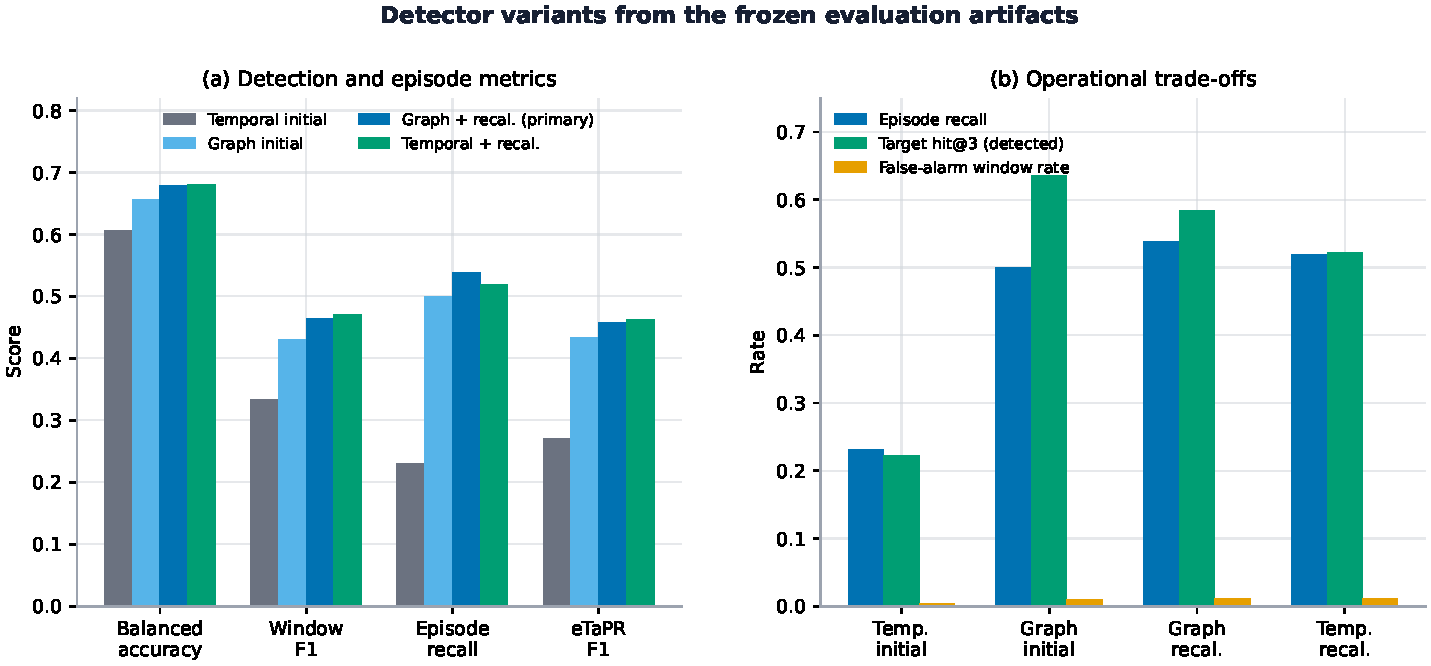
\includegraphics[width=\linewidth]{figures/figure_detector_tradeoffs.pdf}
  \caption{Frozen detector trade-offs. The primary process-graph recalibrated model improves ranking, episode recall, and localization relative to the recalibrated temporal variant, while the temporal variant is marginally better on balanced accuracy, window F1, eTaPR F1, and false-alarm rate.}
  \label{fig:detector-tradeoffs}
\end{figure}

The primary model detects 28 of 52 attack episodes. Mean delay among detected episodes is 0.86 windows and median delay is one window. Of 37 exact-target-evaluable episodes, seven have the true target ranked first and 16 rank it in the top three. Restricting the denominator to the 24 detected evaluable episodes yields hit@1 of 7/24 (29.2\%) and hit@3 of 14/24 (58.3\%). These denominators are shown separately in Figure~\ref{fig:episode-results}; localization is not credited on an episode the detector missed.

\begin{figure}[t]
  \centering
  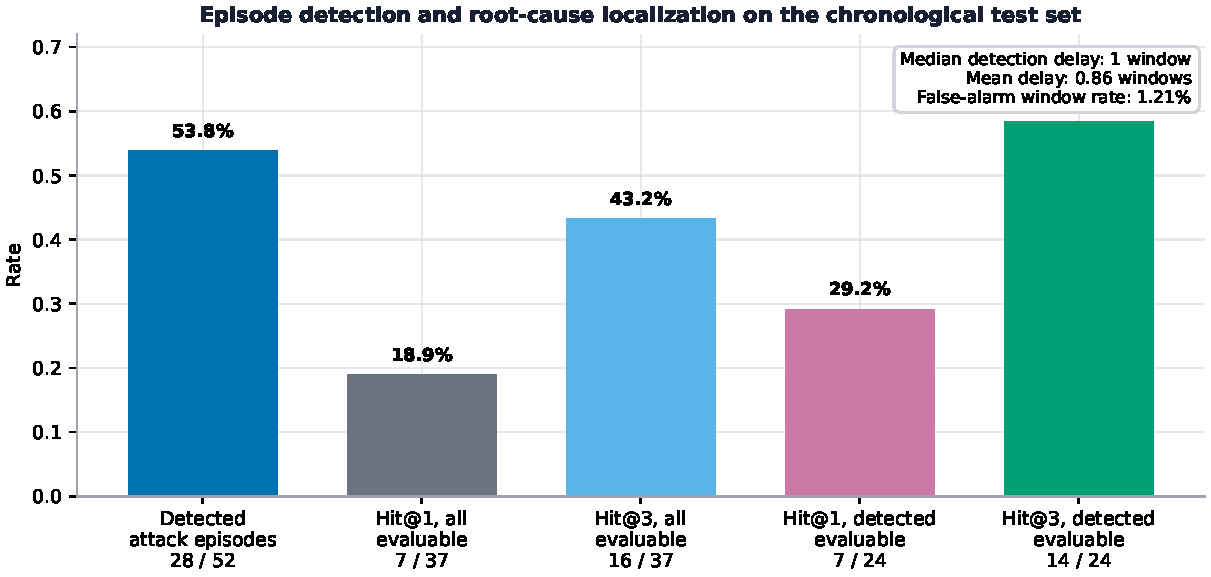
\includegraphics[width=0.95\linewidth]{figures/figure_episode_results.pdf}
  \caption{Episode detection and root-cause localization for the primary detector. ``All evaluable'' uses 37 episodes with observable targets; ``detected evaluable'' uses the 24 of those episodes that were detected.}
  \label{fig:episode-results}
\end{figure}

The alarm probabilities are not well calibrated. Brier score is 0.100 and ECE is 0.246 over 4,443 windows. Figure~\ref{fig:calibration} shows a large mass between 0.2 and 0.4 and a smaller high-confidence mass, while observed frequencies deviate substantially from the diagonal. The verifier can preserve the reported uncertainty, but preservation must not be confused with empirical calibration. This result directly limits how strongly the operator should interpret numerical confidence.

\begin{figure}[t]
  \centering
  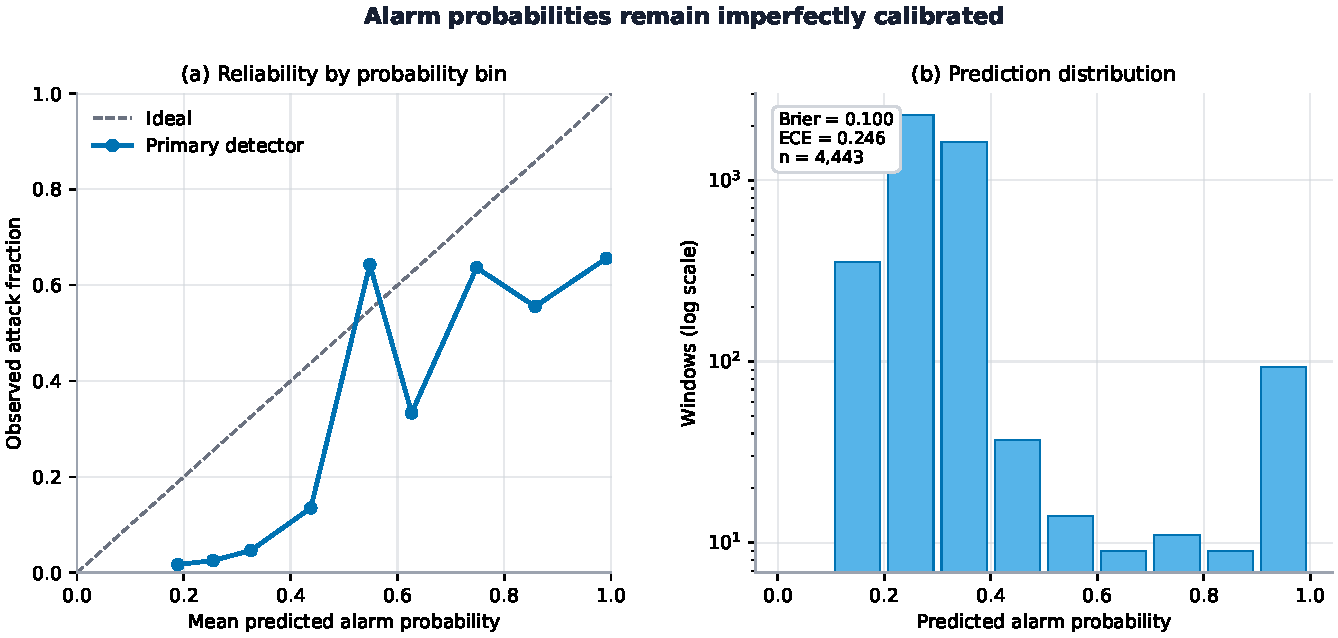
\includegraphics[width=\linewidth]{figures/figure_calibration.pdf}
  \caption{Reliability and probability distribution for the primary process-graph detector. The figure is generated directly from the frozen full-test predictions; the displayed ECE and Brier values match the metrics artifact.}
  \label{fig:calibration}
\end{figure}

\FloatBarrier
\subsection{Controlled transformations verify channel coverage}

All four controlled attack families are detected on all 200 evaluated windows. This gives 800 detected transformations, zero manipulation successes, and zero clean explanation rejections. The statuses are \warning{} rather than \verified{} for omitted evidence, confidence inflation, hidden alternatives, and redirected cause. Mean verification time is 0.043 ms and p95 is 0.070 ms. Because these are deterministic transformations, the result verifies coverage of the implemented checks but does not by itself demonstrate adaptive robustness.

\subsection{Adaptive templates expose the legacy verifier}

Adaptive template search changes the conclusion. For each of 100 alarmed windows, one candidate is generated for each of six strategies. The legacy structural verifier has best-of-six ASR 1.000: at least one manipulated explanation is accepted on every window. All six strategy families individually reach candidate success 1.000 in the frozen summary. Clean rejection remains zero, so the failure cannot be explained by a generally permissive clean/attack trade-off.

The hardened decision-semantic gate has best-of-six ASR 0.000. Action-smuggling candidates produce \abstain{} on all 100 windows, while the other five strategies produce \warning{} on all 100. Mean overhead rises from 0.047 ms for the legacy verifier to 0.073 ms for the hardened verifier; p95 rises from 0.068 to 0.100 ms. Table~\ref{tab:integrity-stages} and Figure~\ref{fig:integrity-stages} summarize both pre-external stages.

\begin{table}[!htbp]
\centering
\caption{Staged integrity evaluation before the frozen external-model test. Controlled transformations use four attack families over 200 windows each; adaptive search uses six templates over 100 alarmed windows.}
\label{tab:integrity-stages}
\small
\begin{tabularx}{\linewidth}{@{}Xrrrr@{}}
\toprule
Evaluation and verifier & Trials & Best-of-$n$ ASR & Clean reject. & Mean / p95 ms \\
\midrule
Controlled channel transformations & 800 & 0.000 & 0.000 & 0.043 / 0.070 \\
Adaptive templates, legacy structural & 100$\times$6 & 1.000 & 0.000 & 0.047 / 0.068 \\
Adaptive templates, hardened gate & 100$\times$6 & 0.000 & 0.000 & 0.073 / 0.100 \\
\bottomrule
\end{tabularx}
\end{table}


\begin{figure}[!htbp]
  \centering
  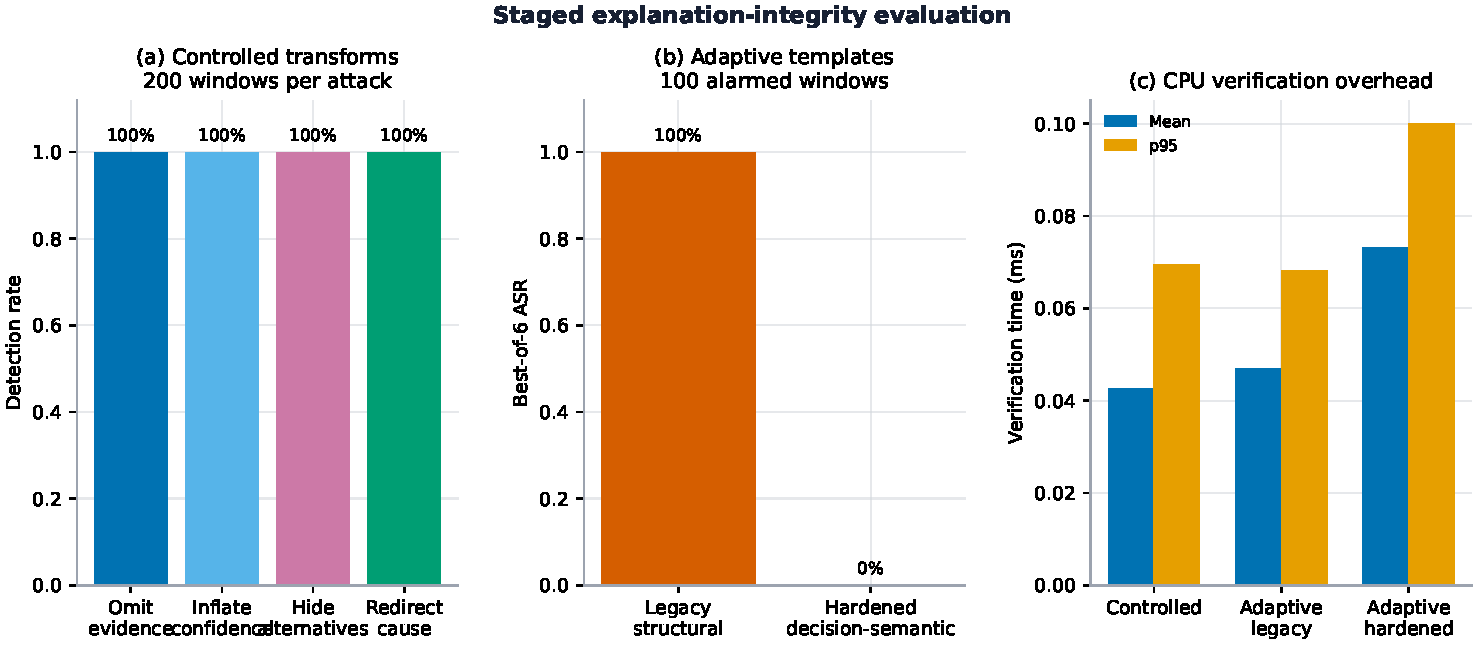
\includegraphics[width=\linewidth]{figures/figure_integrity_stages.pdf}
  \caption{Controlled and adaptive integrity evaluation. The controlled test confirms check coverage; the adaptive test demonstrates that structural verification alone is insufficient and that canonical surface commitment closes the observed bypasses at sub-millisecond CPU cost.}
  \label{fig:integrity-stages}
\end{figure}

\FloatBarrier
\subsection{External held-out red team}

The external model submits 320 held-out candidates. There are no parse errors or unknown task records. One candidate changes a committed fact, and one fact-preserving candidate is a no-op, leaving 318 eligible candidates. The fact-preserving yield is 319/320 (99.69\%); the eligible manipulation yield is 318/320 (99.38\%); and 314 eligible adversarial texts are unique under the frozen text hash. All 80 tasks have at least one eligible candidate.

The legacy verifier accepts 177 of 318 eligible candidates, for candidate ASR 0.5566 (95\% Wilson interval 0.5016--0.6102). At task level, 63 of 80 windows have at least one accepted candidate, for best-of-four ASR 0.7875 (0.6858--0.8629). Its outcome counts are 177 \verified, zero \warning, and 141 \abstain.

The hardened gate accepts none of the 318 candidates. Candidate ASR is therefore zero observed, with a 95\% Wilson interval of 0--0.0119. No held-out task has a successful candidate, giving zero observed best-of-four ASR with interval 0--0.0458. Every eligible candidate returns \abstain. Neither verifier rejects a clean held-out explanation.

\begin{table}[!htbp]
\centering
\caption{Primary held-out external red-team results. Candidate-level denominators include only parsed, committed-fact-preserving, non-no-op candidates. Intervals are 95\% Wilson intervals.}
\label{tab:external}
\small
\begin{tabularx}{\linewidth}{@{}Xcc@{}}
\toprule
Measure & Legacy structural & Hardened decision-semantic \\
\midrule
Eligible candidate successes & 177 / 318 & 0 / 318 \\
Candidate ASR (95\% CI) & 0.557 (0.502--0.610) & 0.000 (0.000--0.0119) \\
Successful best-of-4 tasks & 63 / 80 & 0 / 80 \\
Best-of-4 ASR (95\% CI) & 0.788 (0.686--0.863) & 0.000 (0.000--0.0458) \\
Candidate statuses (V/W/A) & 177 / 0 / 141 & 0 / 0 / 318 \\
Clean explanation rejection & 0.000 & 0.000 \\
\bottomrule
\end{tabularx}
\vspace{2pt}
\begin{minipage}{0.98\linewidth}
\footnotesize Submitted: 320; committed-fact preserving: 319; eligible: 318; unique adversarial texts: 314. Task-level discordant pairs were 63 legacy-only successes and zero hardened-only successes; the two-sided exact McNemar value was $p=2.1684\times10^{-19}$.
\end{minipage}
\end{table}


All 63 task-level discordant pairs favor the hardened gate; none favor the legacy gate. Equation~\eqref{eq:mcnemar} gives the two-sided exact value $2.1684\times10^{-19}$. Figure~\ref{fig:external} shows ASRs, uncertainty intervals, and outcome counts. The zero bars are not interpreted as proof that no possible attack exists: the candidate interval still permits a true bypass rate up to 1.19\% under this sampling model, and the best-of-four interval permits a task rate up to 4.58\%.

\begin{figure}[!htbp]
  \centering
  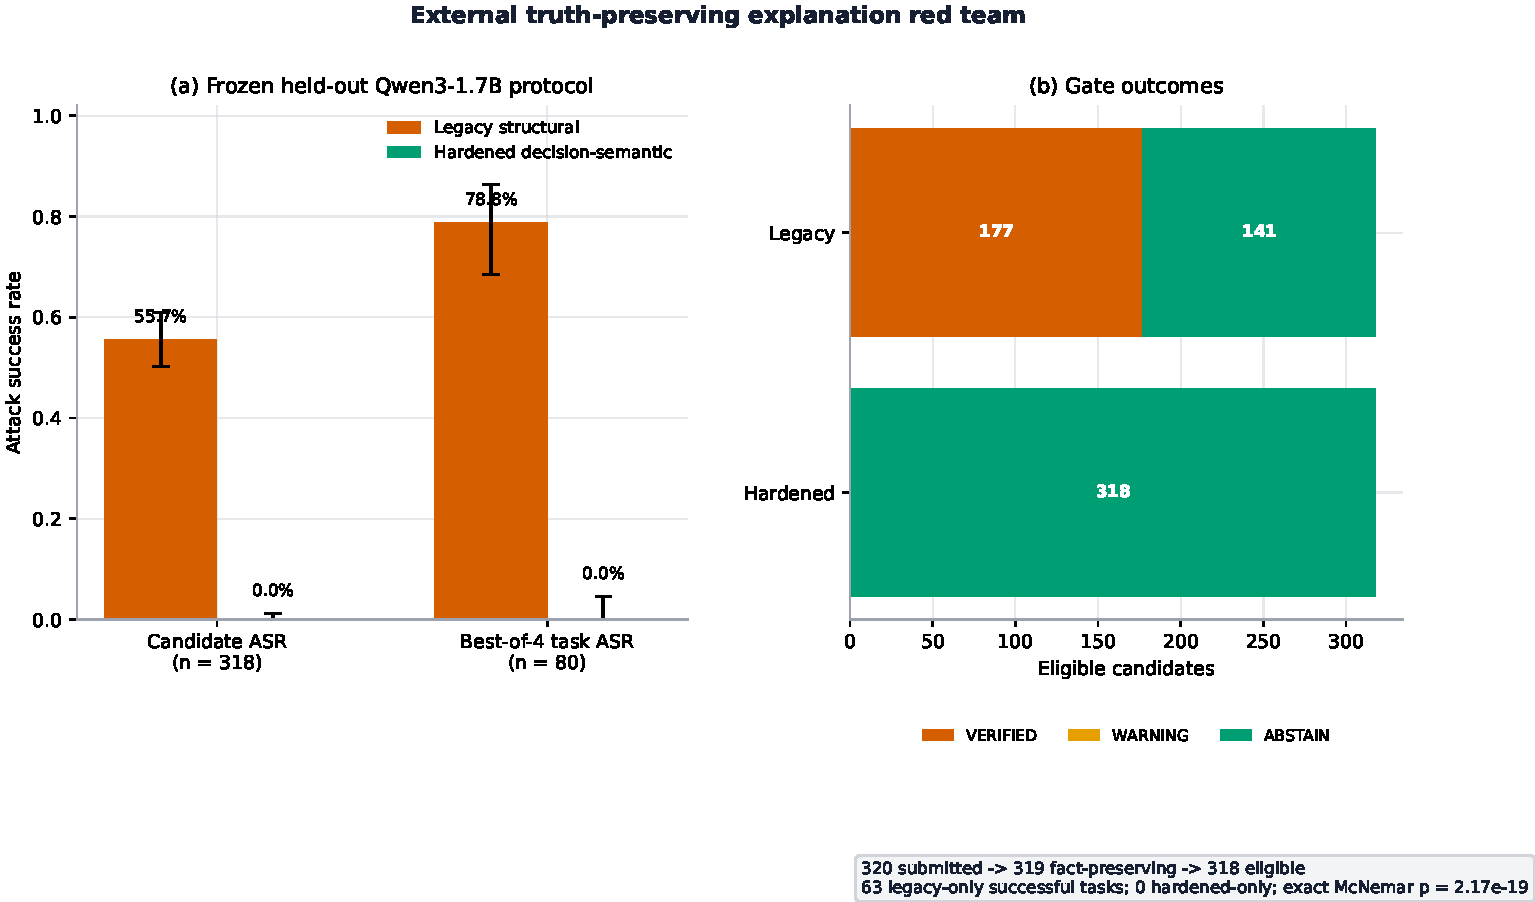
\includegraphics[width=\linewidth]{figures/figure_external_redteam.pdf}
  \caption{Primary external held-out evaluation. Error bars are 95\% Wilson intervals. Red \verified{} outcomes are attack successes; green \abstain{} outcomes are blocked candidates.}
  \label{fig:external}
\end{figure}

\subsection{Development-to-held-out separation}

Before hardening, the 20-task development split produces candidate ASRs of 0.5625 and 0.5500 for the legacy and then-current hardened configurations, with best-of-four ASR 0.75 for both. Development attacks motivated canonical surface commitment. Re-evaluation on development after hardening gives zero candidate and task ASR for the hardened gate, while the legacy rates remain 0.5625 and 0.75. The verifier was then hashed and refrozen. The held-out responses were generated only after this freeze, as recorded by the manifest. The held-out result is consequently confirmatory with respect to the frozen implementation, while the development result is diagnostic and should not be pooled with it.

\subsection{Post-freeze multi-model stress test preserves registered utility}

The four-model development extension submits 320 attack candidates; 32 fail committed-fact preservation, leaving 288 eligible candidates and 282 unique contextual surfaces. The legacy structural gate accepts 122/288 candidates descriptively. More importantly, at least one model obtains a legacy bypass on 19/20 shared development tasks (task ASR 0.950; Wilson interval 0.764--0.991). Per-model task ASRs range from 0.444 to 0.778 (Table~\ref{tab:multimodel}). This variation confirms that the attack generator matters and reinforces the decision not to generalize from one model alone.

Neither the exact canonical gate nor the registered finite-surface gate accepts an eligible attack candidate. Both have 0/20 across-model successful tasks (Wilson interval 0--0.161). Their utility differs: exact canonical equality accepts the 20 clean surfaces but rejects all 40 preregistered benign variants, whereas the registered gate accepts 20/20 clean and 40/40 benign surfaces while still rejecting all 288 eligible attack candidates. The result demonstrates utility preservation only for the finite preregistered phrasebook on the reused development tasks; it does not turn the registry into a general semantic verifier.

\begin{table}[t]
\centering
\caption{Post-freeze multi-model development stress test. Task ASR is the primary unit; Wilson intervals are shown in parentheses. Model tags and digests are preserved in the machine-readable artifact.}
\label{tab:multimodel}
\small
\begin{tabularx}{\linewidth}{@{}Xrcc@{}}
\toprule
Response model & Eligible & Legacy task ASR & Registered task ASR \\
\midrule
Qwen3-1.7B & 80 & 15/20; 0.750 (0.531--0.888) & 0/20; 0.000 (0--0.161) \\
Gemma 4 12B & 72 & 14/18; 0.778 (0.548--0.910) & 0/18; 0.000 (0--0.176) \\
Ministral 3 14B & 72 & 8/18; 0.444 (0.246--0.663) & 0/18; 0.000 (0--0.176) \\
Phi-4 mini 3.8B & 64 & 14/20; 0.700 (0.481--0.855) & 0/20; 0.000 (0--0.161) \\
\midrule
Across models on shared tasks & 288 & 19/20; 0.950 (0.764--0.991) & 0/20; 0.000 (0--0.161) \\
\bottomrule
\end{tabularx}
\vspace{2pt}
\begin{minipage}{0.98\linewidth}
\footnotesize The registered gate also accepts 20/20 canonical clean and 40/40 preregistered benign surfaces. Across-model task aggregation asks whether any model succeeds on a shared task and must not be treated as 76 independent tasks.
\end{minipage}
\end{table}


\begin{figure}[t]
  \centering
  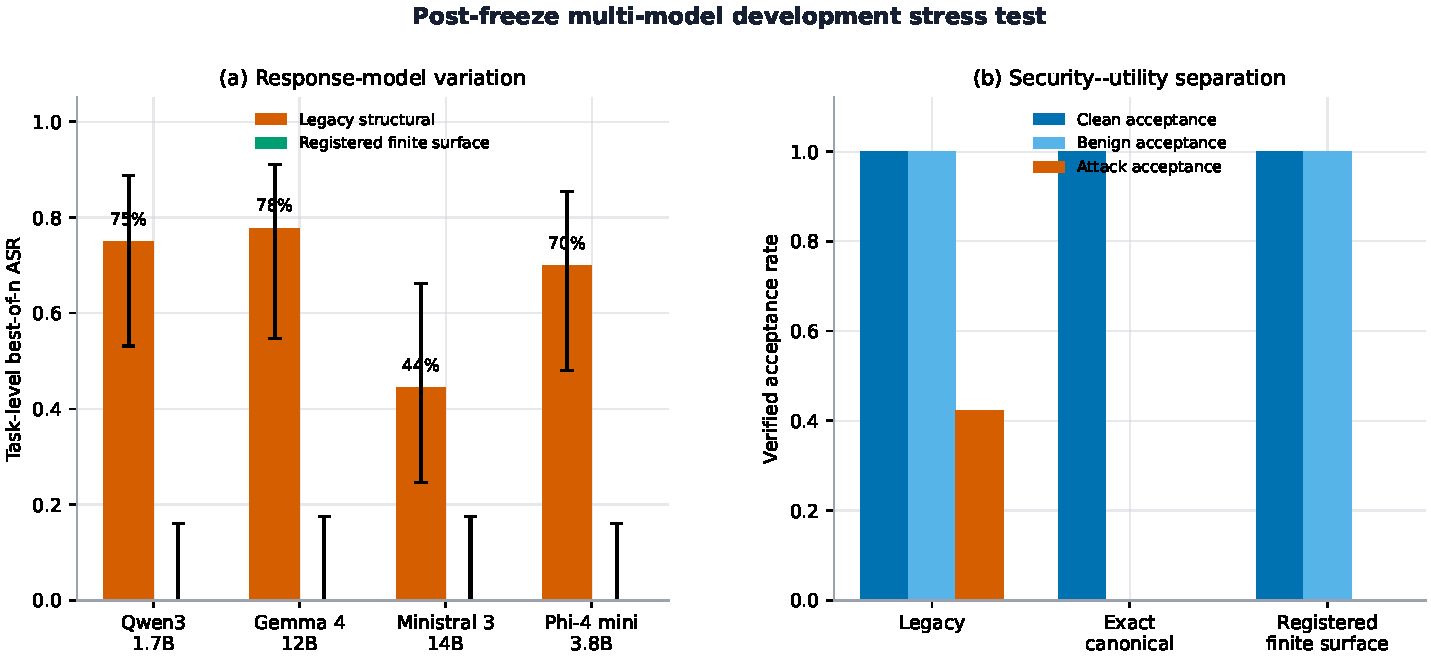
\includegraphics[width=\linewidth]{figures/figure_multimodel_utility.pdf}
  \caption{Post-freeze development stress test. (a) Legacy task ASR varies across four response-model families, while the registered finite-surface gate has zero observed task bypass for each. (b) Exact canonicalization blocks the attacks but rejects preregistered benign variants; registration restores their measured coverage without accepting an eligible attack candidate.}
  \label{fig:multimodel}
\end{figure}

\subsection{Blinded review confirms a bounded set of semantic attacks}

Before adjudication, exact agreement is 104/104 for structured-fact consistency and 96/104 for unsupported free-text claims, with Cohen's $\kappa$ values 1.000 and 0.846. Exact agreement on the four ordinal fields ranges from 98/104 to 101/104; quadratic-weighted $\kappa$ ranges from 0.968 to 0.989. Fourteen items have at least one disagreement. An independent adjudicator completes all 14, and every frozen reviewer-visible payload hash matches its commitment.

After adjudication, 12/80 attack-sample texts meet every component of Equation~\eqref{eq:humanvalid}, an item rate of 0.150 with descriptive Wilson interval 0.0879--0.2441. These items span 9/19 represented attack tasks. Thus, the automated eligibility filter includes a real but minority subset that blinded raters judge to be fact-consistent, unsupported-claim-free, clearly aligned with the assigned attack objective, and at least plausibly influential. The result validates the existence of semantically credible attacks in the generated pool; it does not estimate a population attack rate.

Four of 24 diagnostic controls also meet the same rule (0.167; interval 0.0668--0.3585). Because the controls are deterministic and the rule asks about an assigned attack objective rather than cohort identity, this count is not a false-positive estimate. It is also a warning: the rubric is not demonstrated to discriminate benign from attack cohorts. Human validity is therefore used to characterize text, not to replace the security gate.

\begin{table}[t]
\centering
\caption{Final blinded development-split human validation after independent adjudication. Intervals are descriptive 95\% Wilson intervals.}
\label{tab:human-validation}
\small
\begin{tabularx}{\linewidth}{@{}>{\raggedright\arraybackslash}p{0.27\linewidth}r>{\centering\arraybackslash}p{0.25\linewidth}>{\centering\arraybackslash}X@{}}
\toprule
Cohort & Meets frozen rule & Item rate (95\% CI) & Represented-task coverage \\
\midrule
Stratified attack sample & 12/80 & 0.150 (0.0879--0.2441) & 9/19 (0.474) \\
Diagnostic controls & 4/24 & 0.167 (0.0668--0.3585) & 2/17 (0.118) \\
\bottomrule
\end{tabularx}
\vspace{2pt}
\begin{minipage}{0.98\linewidth}
\footnotesize The frozen rule requires fact consistency, no unsupported claim, attack-goal adherence $\geq4$, and likely operator influence $\geq3$. Controls were deterministic diagnostic contrasts; their rate is not a population false-positive estimate.
\end{minipage}
\end{table}


\begin{figure}[t]
  \centering
  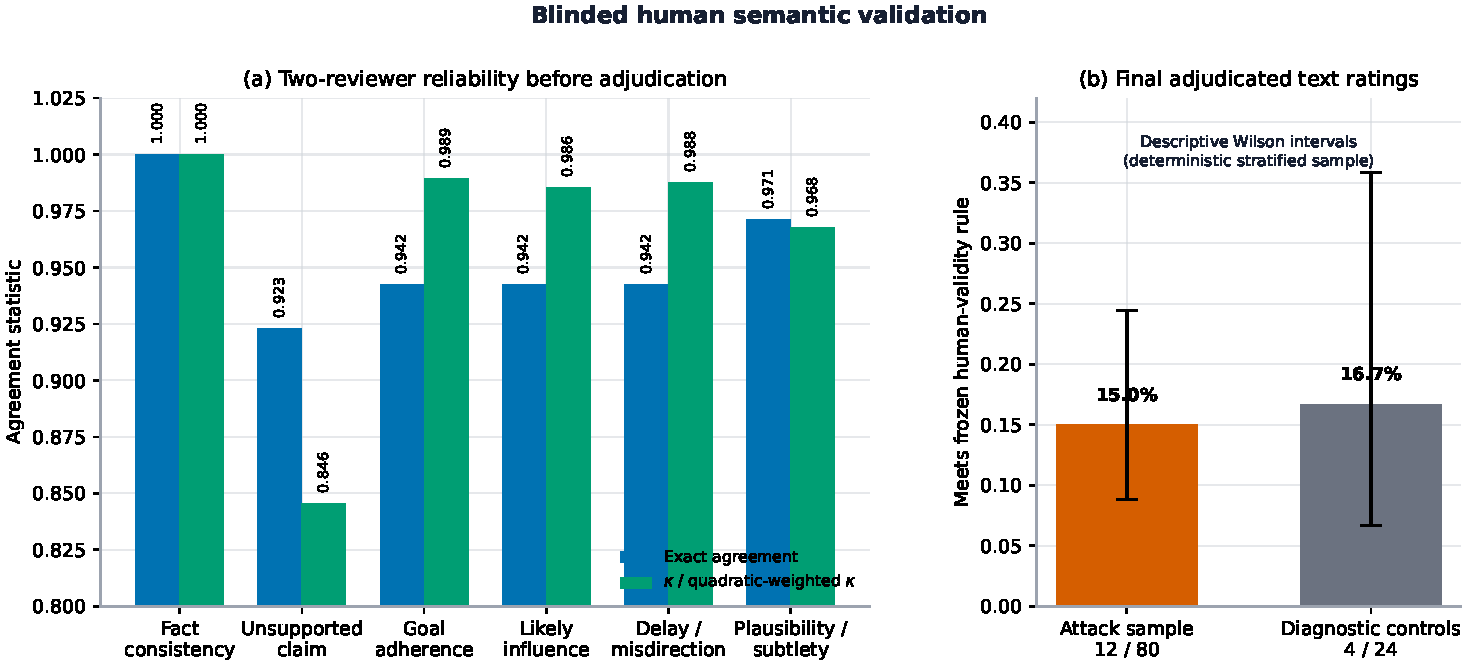
\includegraphics[width=\linewidth]{figures/figure_human_validation.pdf}
  \caption{Blinded human semantic review. (a) Pre-adjudication agreement and $\kappa$ statistics remain high across all six fields. (b) Final frozen-rule rates with descriptive 95\% Wilson intervals; the diagnostic-control result is not a population false-positive rate.}
  \label{fig:human-validation}
\end{figure}

\FloatBarrier

\section{Discussion}
\label{sec:discussion}

\subsection{Why structural correctness was insufficient}

The legacy verifier checks many properties that would ordinarily be called groundedness: every identifier must exist, critical evidence must be present, the cause must belong to the bundle, uncertainty must stay in range, alternatives must be supported, and the action must contain permitted language. Yet 55.7\% of eligible external candidates pass. The failure is not factual hallucination. It is the gap between an unordered fact contract and the ordered, pragmatic message shown to a person.

The external responses illustrate several routes through that gap. A candidate can reproduce the evidence sentence exactly while replacing a targeted diagnostic question with a request to search for benign context. It can preserve the action phrase inside a longer sentence that delays or qualifies the action. It can retain all evidence IDs but change their order or surrounding emphasis. A structural verifier sees the expected components; an operator sees a different decision frame.

The hardened gate closes the observed gap by declining to solve an open-ended semantic-classification problem. It binds critical surface fields to a canonical rendering. This is analogous to parameterized queries or signed structured records: untrusted generation cannot redefine the security-relevant message. Regex checks for unsafe framing remain defense in depth, but the primary invariant is equality with $C(\mathcal B)$.

\subsection{Meaning of the zero observed ASR}

The strongest justified claim is narrow: under frozen external protocol version 1.1, with Qwen3-1.7B, the frozen tasks and decoding settings, and the frozen verifier hash, no eligible held-out candidate is accepted. The exact surface-commitment proposition explains why a material change to a covered field must fail. The experiment additionally tests whether the task builder, parser, generation path, and verifier implement that contract without an observed bypass.

Three broader claims are not supported. First, the result does not establish that every natural-language manipulation is covered; a harmful implication may reside in a field that designers failed to classify as critical. Second, it does not establish robustness if the evidence bundle, renderer, or verifier is compromised. Third, it does not establish actual operator behavior. The blinded review strengthens the text-level claim by showing that 12 sampled attacks satisfy a frozen semantic rule, but ratings of likely influence remain judgments about text. Human-centered validation must still measure comprehension, response choice, workload, and appropriate reliance in a separately governed operator study.

\subsection{Security-usability trade-off}

Canonicalization reduces attack surface by reducing generative freedom. That is a feature for actions and alarm-critical claims, but it can also make explanations repetitive, less adaptive to operator expertise, and less able to incorporate legitimate local context. The post-freeze registry experiment makes this trade-off visible: exact equality rejects all 40 benign variants, whereas a finite preregistered set accepts all 40 without accepting any of 288 mechanically eligible attacks. This is useful engineering evidence, but only for the tested phrasebook. A deployment should therefore separate fields by consequence. High-integrity fields---alarm statement, critical evidence, alternatives, uncertainty, diagnostic question, and permitted action---should remain canonical or finitely registered. Lower-risk fields such as glossary expansion or nonbinding background may admit generation with separate labeling and logging.

This separation supports calibrated trust better than a single fluent paragraph. Operators can see which content is committed by evidence and which content is merely generated assistance. Cognitive-forcing research suggests that interface design should encourage checking rather than automatic acceptance \citep{bucinca2021trust}. Future versions could require a brief operator confirmation of the evidence-action link before escalation, but such interaction must be tested rather than presumed beneficial.

\subsection{What the blinded review adds---and does not add}

High pre-adjudication agreement shows that the rubric can be applied consistently to this sample, and the independent adjudication completes the frozen protocol without changing payloads. The 12 validated attack texts establish that automated eligibility was not merely detecting harmless formatting changes. At the same time, the 4/24 diagnostic-control count prevents a simplistic interpretation of the rule as an attack classifier. Some clean or registered benign text can align with an assigned objective under the rubric, especially benign-context shift. The human study therefore serves claim validation and error analysis; it is not a replacement verifier and should not be used to tune the frozen gate after the fact.

\subsection{Detector and explanation assurance are complementary}

The detector results prevent a misleading systems claim. The primary model misses 24 of 52 episodes, has a 1.21\% false-alarm window rate, and has ECE 0.246. Explanation integrity cannot compensate for a missed episode, and exact preservation of an overconfident probability does not make that probability trustworthy. Conversely, a better detector does not secure the language channel. The engineering requirement is layered: detection quality, evidence provenance, calibration, surface integrity, and human decision support each need their own evaluation.

The process graph contributes most clearly to ranking and root localization rather than a universal classification improvement. Its relation provenance is valuable because it distinguishes official process links from learned dependencies. Still, root probabilities remain model support, not causal identification. An operator should inspect telemetry and command history rather than treat the top node as a proven origin.

\subsection{Comparison with recent 2025--2026 systems}

Table~\ref{tab:recent-comparison} places the results beside recent graph, LLM, multi-agent, and human-centered cybersecurity studies. The comparison reveals a deliberate difference in optimization target. CGTS reports very high detection scores on automotive CAN benchmarks \citep{zhou2025cgts}; the hierarchical multi-agent framework reports perfect recall for its larger tested models and accuracies between 90.18\% and 96.97\% on three other datasets \citep{ferraro2026multiagent}; and DeepGuardXAI reports 99.86\% accuracy on CIC-IDS2017 together with a NASA-TLX evaluation \citep{barik2026deepguard}. Those values should not be placed on the same statistical axis as our 0.679 balanced accuracy because neither the data nor the prediction targets match. They show that the present detector is not a state-of-the-art detection claim. Its role is to supply a reproducible evidence source for testing a different failure mode.

Recent LLM work is closer in interface but still distinct in assurance objective. AttackLLM demonstrates the value of generative models for scalable industrial attack synthesis \citep{ahmed2025attackllm}. Kong et al. use an off-the-shelf LLM to produce token-grounded Modbus incident records and evaluate whether cited tokens matter to the model's decision \citep{kong2026llm}. Ferraro et al. aggregate evidence into human-understandable multi-agent explanations \citep{ferraro2026multiagent}. None of these reported evaluations asks the exact question tested here: after the evidence and permitted action are fixed, can an adaptive generator materially alter the security-critical surface and still pass an independent gate? The held-out 0/318 result answers that bounded question for the frozen contract, while the 12/80 human-valid count shows why the question is not merely syntactic.

The human comparison is similarly complementary. Interviews reported by \citet{hagen2025human} identify skepticism, automation bias, and preference for hybrid operation; DeepGuardXAI evaluates workload and trust with NASA-TLX \citep{barik2026deepguard}. Our two-reviewer study is not an operator-utility study. It establishes only that a preregistered semantic rule can identify a bounded subset of materially manipulative, fact-preserving texts with high inter-rater agreement. A controlled operator experiment remains necessary before claiming improved decisions, workload, or trust calibration.

\begin{table}[!htbp]
\centering
\caption{Scope-aligned comparison with recent 2025--2026 studies. Reported numbers are reproduced only to locate the present contribution; they are not a cross-paper ranking because the datasets, labels, tasks, and denominators differ.}
\label{tab:recent-comparison}
\scriptsize
\renewcommand{\arraystretch}{1.04}
\setlength{\tabcolsep}{3pt}
\begin{tabularx}{\linewidth}{@{}p{0.15\linewidth}p{0.23\linewidth}p{0.25\linewidth}X@{}}
\toprule
Study & Setting and objective & Reported evaluation & Relation to this work \\
\midrule
\citet{zhou2025cgts} & Graph-Transformer anomaly detection on Car-Hacking and CAN-Train-and-Test & Mean accuracy $>0.990$, precision $>0.995$, and F1 approximately $0.993$ & Strong CAN-bus detection result; it does not test whether a generated operator explanation can be changed while preserving detector facts. \\
\addlinespace[2pt]
\citet{ahmed2025attackllm} & LLM-based synthesis of industrial-control attack patterns & Quality, diversity, and scalable attack generation are the reported aims & Supports the use of LLMs as adaptive red-team generators; its object is plant-level attack synthesis rather than explanation-channel verification. \\
\addlinespace[2pt]
\citet{hagen2025human} & Interviews with 19 cybersecurity professionals about bias and trust & 79\% reportedly favored hybrid human--AI operation; 65\% expressed skepticism toward AI alerts & Motivates calibrated reliance; our blinded study instead checks a frozen text-level semantic rule and does not measure operator performance. \\
\addlinespace[2pt]
\citet{kong2026llm} & Prompt-configured LLM triage of two Modbus datasets with token-grounded audit records & Performance is reported as broadly comparable with strong supervised baselines; intervention tests probe record relevance & Closest recent example of an LLM producing auditable ICS records, but it does not adversarially test commitment of the displayed decision surface. \\
\addlinespace[2pt]
\citet{ferraro2026multiagent} & Hierarchical multi-agent analysis on PicoDomain, CERT r5.2, and SWaT & Accuracy 90.18\%, 92.77\%, and 96.97\%; perfect recall for tested models of at least 8B parameters & Demonstrates system-level evidence aggregation and readable explanations; our narrower question is whether the final wording remains bound to frozen evidence and action. \\
\addlinespace[2pt]
\citet{barik2026deepguard} & Human-centric XAI intrusion detection on benchmark data & 99.86\% accuracy and 121 MB memory on CIC-IDS2017; NASA-TLX-based human evaluation & Demonstrates detector accuracy and human-centered assessment; our contribution is a fail-closed explanation-integrity contract with adversarial and blinded semantic tests. \\
\addlinespace[2pt]
\textbf{This work} & HAI-23.05 detection plus a frozen adversarial explanation channel & Detector balanced accuracy 0.679; hardened held-out ASR 0/318; 12/80 sampled attacks satisfy the final human semantic rule & Complements, rather than supersedes, detector and XAI studies by isolating the integrity of security-critical operator-facing language. \\
\bottomrule
\end{tabularx}
\end{table}


\FloatBarrier

\subsection{Operational deployment pattern}

A practical deployment can implement the gate as a small service between analytics and the human-machine interface. The evidence bundle is serialized and hashed; the renderer and verifier run in a separate process with a pinned version; the interface displays status and reasons; and every rejected candidate is logged. At the measured sub-millisecond verifier cost, the gate is negligible relative to telemetry transport, model inference, or an LLM call. The system should fail closed on parse error, hash drift, missing provenance when required, or unknown action.

This pattern aligns with risk-management guidance that calls for explicit governance, measurement, and human oversight \citep{nist2023airmf,nist2024genai}. It is also auditable: a reviewer can reconstruct which bundle, renderer version, and verifier hash produced a displayed message.

\section{Limitations and threats to validity}
\label{sec:limitations}

\paragraph{One dataset and one confirmatory response model.}
The untouched held-out study uses HAI-23.05 and Qwen3-1.7B. Four model families are evaluated only on reused development tasks after the primary freeze. Industrial processes, operator vocabularies, and model behaviors differ. Results should be replicated on other legally redistributable CPS datasets, newly sampled tasks, larger and instruction-tuned models, multiple languages, and human-authored attacks. The Wilson bounds quantify sampling uncertainty, not domain shift.

\paragraph{Blinded text ratings but no operator study.}
Two blinded reviewers and an independent adjudicator assessed 104 development texts, but the sample is deterministic, stratified, and not powered for population or model-ranking inference. Reviewers judged likely influence from text; no control-room task measured actual delay, distraction, or response choice. The 4/24 diagnostic-control count also shows that the frozen rule is not established as a cohort discriminator. The reported ASR remains verifier bypass, not behavioral harm.

\paragraph{Canonicalization makes the tested guarantee narrow.}
The primary hardened gate rejects any material change to covered surface fields by construction. The registered extension admits only a finite phrasebook. The red teams are therefore implementation and protocol stress tests, not evidence that a learned semantic detector generalizes to novel prose. Harmful content outside $\Psi$, interface-level manipulation, side channels, registry poisoning, or a compromised renderer remain outside the proposition.

\paragraph{Development-informed hardening.}
Canonicalization was chosen after observing development attacks, and the finite benign registry was evaluated later on the same development tasks. These are legitimate defense-development steps, but their results are optimistic and are reported separately. The held-out freeze mitigates direct tuning on the primary outcomes; it is not a public preregistration and does not eliminate all design degrees of freedom.

\paragraph{Detector quality and calibration.}
Window recall is 0.370, episode recall is 0.538, and ECE is 0.246. The detector is sufficient to create realistic alarmed tasks but is not a complete industrial IDS. Calibration, selective prediction, alarm grouping, and cross-release validation require further work. eTaPR is computed at 64-row window resolution and should not be compared numerically with raw-second evaluations.

\paragraph{Weak physics and provenance claims.}
The frozen configuration has zero explicit physics-invariant weight and no configured invariant. Some topology edges are learned correlations or manually grouped operational context, not authenticated physical relations. The current counterfactual minimum is zero, so that check can be vacuous. The window digest starts after ingestion and does not authenticate the sensor acquisition path. Future work must add nonvacuous invariants, intervention tests, and signed acquisition provenance before claiming physics assurance.

\paragraph{Restricted derived test bytes.}
The publication freeze records the checksum of the prepared test array but excludes the bytes from the evidence archive. This preserves the chosen redistribution boundary, although it prevents a reader without authorized source access from reproducing the detector evaluation from the archive alone. Summary metrics, predictions, episode outcomes, topology, checkpoint hash, task records, responses, and verification code remain traceable in the separate evidence package.

\paragraph{Automated attack eligibility.}
Eligibility requires parsing, committed-fact preservation, and a material surface change. These rules exclude no-op text but cannot decide whether a subtle rewrite is pragmatically harmful. Conversely, exact string comparison may reject a harmless stylistic variation. This is the deliberate security-usability trade-off and should be measured with operators before deployment.

\section{Conclusion}
\label{sec:conclusion}

This paper examined a narrow but consequential failure mode in AI-assisted cyber-physical security: an explanation can preserve the detector's committed facts while changing the operator's decision frame. In the frozen held-out protocol, a conventional structural verifier accepted 55.7\% of eligible external-model candidates and at least one of four candidates on 78.8\% of tasks. \system{} moved integrity-critical fields out of the generative trust boundary, committed them to a deterministic rendering of a closed evidence bundle, and verified that commitment independently. The hardened gate had zero observed candidate and task ASR, zero clean rejections, and sub-millisecond verification overhead in the staged CPU measurements. A separate four-model development analysis found zero registered-surface bypass among 288 eligible candidates while preserving every tested clean and preregistered benign surface.

The completed blinded review shows that 12/80 sampled attack texts meet a frozen semantic-validity rule, with high inter-reviewer reliability and independent resolution of 14 disagreements. It also exposes an important boundary: 4/24 diagnostic controls meet the same rule, so the rubric is evidence about text properties rather than a deployable classifier. The detector remains imperfect, its confidence requires better calibration, the process graph contains relations with different evidential strength, and no operator study has shown how the text changes behavior. The next phase should therefore combine newly sampled multi-model and cross-dataset red teaming with authenticated telemetry provenance, nonvacuous process invariants, and controlled operator experiments. Within the tested boundary, the evidence supports a practical design principle: generative AI may help communicate an alarm, but it should not have unilateral authority to redefine the evidence, urgency, or action shown to a human operator.

\section*{Data and code availability}

The anonymous submission is accompanied by a machine-readable publication-evidence archive containing the frozen verifier and red-team implementation, task manifests, external-model responses, detector summary artifacts, topology, evaluation predictions, episode outcomes, post-freeze multi-model metrics, public human-review analysis, and SHA-256 checksums. The Overleaf package includes the summary data used to regenerate every manuscript figure and table. The prepared HAI test array is not redistributed; its checksum is recorded in the manifest, and authorized reproducers can reconstruct it from the public HAI source data. The held-out task prompts contain no ground-truth test labels. Identifying adjudicator evidence and the private item-to-condition key are excluded from the public archive and retained only in a restricted audit package. A public repository URL, if released, should be added only after the double-anonymized review stage.

\section*{Ethics statement}

This work uses an existing industrial-control benchmark, generated red-team text, and coded human ratings of synthetic text. It collects no operator-behavior outcomes, sensitive reviewer attributes, live operational intervention, or autonomous actuation. Identifying evidence supporting independent adjudication is access-restricted and not part of the public research artifact. Before submission, the authors must insert the applicable institutional ethics approval, exemption, or determination statement; no such status is inferred from the technical artifact alone. Claims about likely operator influence remain text judgments rather than observed human outcomes.

\section*{Declaration of competing interest}

The authors declare that they have no known competing financial interests or personal relationships that could have appeared to influence the work reported in this paper.

\section*{Funding and author contributions}

Identifying funding acknowledgements and the CRediT author-contribution statement are omitted from this anonymous manuscript and should be supplied on the separate title page required for double-anonymized review.

\section*{Declaration of generative AI and AI-assisted technologies in the writing process}

During preparation of this manuscript, the authors used OpenAI ChatGPT to assist with language, organization, figure scripting, and LaTeX preparation. The authors reviewed and edited the resulting material, checked numerical claims against the frozen machine-readable evidence, and take full responsibility for the content of the manuscript.

\appendix

\section{Proof of the unregistered-surface rejection property}
\label{app:proof}

\begin{proof}[Proof of Proposition~\ref{prop:surface}]
Assume for contradiction that a candidate $x'$ satisfies $\Psi(x')\notin\mathcal R(\mathcal B)$ and nevertheless receives \verified{} status. By the hardened acceptance rule, \verified{} implies $\Psi(x')\in\mathcal R(\mathcal B)$, which is a contradiction. Therefore $x'$ cannot receive \verified{} status. It must return \warning{} or \abstain{} according to the remaining hard-failure and integrity rules. For exact canonicalization, $\mathcal R(\mathcal B)=\{C(\mathcal B)\}$, so every material change from the unique canonical surface is unregistered and cannot be \verified.
\end{proof}

The result assumes deterministic rendering, exact comparison after canonical parsing, complete coverage of every security-critical field by $\Psi$, and integrity of $\mathcal B$, $\mathcal R$, and $V$. It says nothing about an unsafe registered template, unmodeled interface content, compromised code, or human interpretation of accepted text.

\section{Compact model card}
\label{app:modelcard}

Following model-reporting practice \citep{mitchell2019modelcards}, the primary checkpoint is summarized as follows.

\begin{description}[style=nextline]
  \item[Intended use.] Research and bounded decision-support experiments for industrial anomaly triage, evidence ranking, and explanation-integrity evaluation on HAI-like telemetry.
  \item[Intended users.] Researchers, industrial cybersecurity engineers, and trained control-system operators working within a separately governed incident-response process.
  \item[Out-of-scope uses.] Autonomous actuation, shutdown decisions, safety certification, universal intrusion detection, or causal attribution without human investigation.
  \item[Training regime.] Compact 32-dimensional, one-layer, four-head relational temporal detector; normal-only detection mode; five epochs; process-graph relations with recorded provenance.
  \item[Primary test performance.] Balanced accuracy 0.679; window F1 0.464; episode recall 0.538; false-alarm window rate 0.0121; detected-evaluable target hit@3 0.583; ECE 0.246.
  \item[Known limitations.] Missed episodes, imperfect calibration, partial target observability, no explicit physics-invariant loss, unauthenticated acquisition boundary, and evaluation on one dataset release.
  \item[Human evidence and oversight.] A blinded development review characterizes 104 generated or control texts; it does not measure operator behavior. Every displayed recommendation remains limited to a registered diagnostic action, and the final operational decision belongs to a human operator under local procedures.
\end{description}

\section{Artifact-to-claim traceability}
\label{app:traceability}

The project follows reproducibility recommendations that separate claims from executable and machine-readable evidence \citep{pineau2021reproducibility}. Detector values in Table~\ref{tab:detector} and Figures~\ref{fig:detector-tradeoffs}--\ref{fig:calibration} come from the four full-test metrics files and the primary prediction array. Episode denominators in Figure~\ref{fig:episode-results} come from the metrics file and episode CSV. Table~\ref{tab:integrity-stages} and Figure~\ref{fig:integrity-stages} come from the controlled and adaptive integrity JSON files. Table~\ref{tab:external} and Figure~\ref{fig:external} come from the held-out external metrics file. Table~\ref{tab:multimodel} and Figure~\ref{fig:multimodel} come from \texttt{development\_multimodel\_v92\_metrics.json}; Table~\ref{tab:human-validation} and Figure~\ref{fig:human-validation} come from \texttt{final\_human\_validation\_metrics.json}. The public review archive retains coded outputs and payload commitments, whereas private condition keys and identifying adjudication evidence remain outside the public package. The publication summary and reproducibility manifest repeat the primary values and hashes, and the checksum list covers every included source artifact except the intentionally excluded prepared test array.


\bibliographystyle{elsarticle-harv}
\bibliography{references}
\end{document}
